%17.09.03


\chapter{Stochastische Geometrie gemischter Perkolation}
\label{sec:mixed}

Im vorangehenden Kapitel wurden Methoden vorgestellt, mit denen die Euler-Charak\-teris\-tik von site-Perkolationsprozessen auf Gittern berechnet werden kann. Wenn aber statt der reinen site-Perkolation gemischte Perkolation betrachtet wird, versagen diese Ans\"atze. Als gemischte Perkolationsprozesse bezeichnen wir solche, die nicht reine site- oder bond-Perkolationsprozesse sind. Zu gemischten Perkolationsprozessen geh\"ort nicht nur bond-site-Perkolation, sondern auch Prozesse, bei denen h\"oherdimensionale Zellen, z.B. Plaketten eines zweidimensionalen Gitters, mit gewissen Wahrscheinlichkeiten ``besetzt'' werden. Vertices auf dem Rand einer solchen besetzten Zelle gelten dann als verbunden. Besetzen der Plaketten eines zweidimensionalen Gitter entspricht der Dekoration (siehe \ref{sec:chimittel}) der Plaketten.
\\Im Laufe der Arbeit habe ich eine Methode entwickelt, mit der geometrische Gr\"o"sen wie die Euler-Charakteristik oder die Oberfl\"ache der Cluster, wie sie bei gemischten Perkolationsprozessen entstehen, berechnet werden k\"onnen. 


\section{Gemischte Perkolation in zwei Dimensionen}
\label{sec:2dmixed}
Wir betrachten ein zweidimensionales planares Gitter, dessen Vertices mit Wahrscheinlichkeit $p_s$ und dessen Kanten mit Wahrscheinlichkeit $p_b$ besetzt sind. Alle Vertices auf dem Rand einer Plakette sind mit Wahrscheinlichkeit $p_f$ verbunden, d.h. die Plakette ist mit Wahrscheinlichkeit $p_f$ dekoriert. F\"ur die dadurch entstehenden Gitterkonfigurationen definieren wir Cluster und berechnen deren geometrische Eigenschaften.  Eine m\"ogliche Konfiguration auf einem Ausschnitt des Quadratgitters ist links in Abbildung \ref{fig:mixed} dargestellt. Bevor die geometrischen Gr\"o"sen einer solchen Konfiguration ausgerechnet werden k\"onnen, m\"ussen die geometrischen Objekte, die den Clustern der Konfiguration entsprechen sollen, festgelegt werden. In unserem Modell treten Cluster nur in Verbindung mit besetzten Vertices auf, und besetzte Kanten oder dekorierte Plaketten, die nur von unbesetzten Vertices umgeben sind, bilden keine Cluster. F\"ur Anwendungen, in denen Kanten und Plaketten Konstituenten verbinden, wie z.B. die Gelbildung aus Monomeren, ist diese Definition sinnvoll. Ob in anderen Anwendungen reine bond-Cluster n\"otig sind, vermag ich nicht zu sagen. In der Graphentheorie versteht man unter dem L\"oschen eines Vertex die Entfernung des Vertex und aller Kanten, die an diesem Vertex enden. Es treten also nie isolierte Kanten auf, in \"Ubereinstimmung mit den hier konstruierten Clustern. Die Forderung, dass Cluster nur in Verbindung mit besetzten Vertices auftreten, f\"uhrt dazu, dass die Konstruktion der geometrischen Objekte, die den Clustern entsprechen sollen, bei den Vertices begonnen werden muss, dann an den Kanten fortgesetzt wird, und dass zum Schluss die Beitr\"age der Plaketten hinzugef\"ugt werden. 
\\Die Figur, die den Gitterclustern entsprechen soll, wird aus den offenen dualen Plaketten, den randlosen dualen Kanten und den dualen Vertices konstruiert. Jeder Vertex des urspr\"unglichen Gitters geh\"ort zu einer dualen Plakette, jede Kante zu einer dualen Kante und jede Plakette zu einem dualen Vertex.
\begin{figure}[tbp]
  \centering
  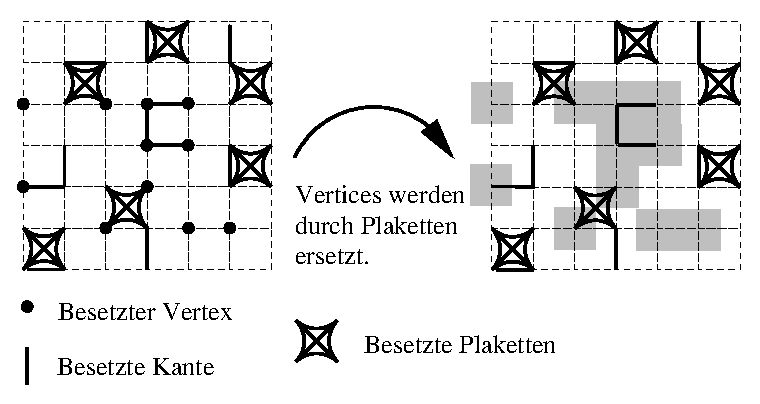
\includegraphics{./Mixed-figs/mixed}
  \caption{Links ist eine m\"ogliche Konfiguration eines gemischten Perkolationsprozesses auf dem Quadratgitter dargestellt. Die Konfiguration enth\"alt auch isolierte Kanten, die keine Cluster bilden. Im ersten Schritt werden auf besetzte Vertices offene duale Quadrate gesetzt (rechts). Damit aus diesen Quadraten Figuren entstehen, die den Gitterclustern entsprechen, m\"ussen sie an den Kanten und Ecken in geeigneter Weise zusammengef\"ugt werden. }
  \label{fig:mixed}
\end{figure}
Die Konfiguration des urspr\"unglichen Gitters beschreiben wir, indem wir jedem Vertex $v$, jeder Kante $k$ und jeder Plakette $f$ eine Variable $\sigma(v)$, $\sigma(k)$ bzw. $\sigma(f)$ zuweisen, die jeweils die Werte $0$ und $1$ annehmen kann. Ist $\sigma=1$, ist der entsprechende Teil des Gitters besetzt. Um die Figuren auf dem dualen Gitter zu beschreiben, f\"uhren wir zu jeder dualen Plakette, jeder dualen Kante und jedem dualen Vertex eine weitere Variable $\lambda(c)$ ein, wobei $c$ die entsprechende Zelle des urspr\"unglichen Gitters bezeichnet.
\\Wir geben die $\sigma$'s auf dem urspr\"unglichen Gitter vor, und konstruieren aus den offenen dualen Zellen eine Figur, die den Gitterclustern entspricht. Jede Plakette des dualen Gitters geh\"ort zur Figur, wenn der Vertex $v$ des urspr\"unglichen Gitters besetzt ist, d.h. $\lambda(v)=\sigma(v)$. Dieser Schritt ist in Abb. \ref{fig:mixed} f\"ur einen Ausschnitt des Quadratgitters illustriert. Die geometrische Figur $F$ besteht nach diesem Schritt aus allen offenen Plaketten mit $\lambda(v)=1$. $F$ wird in den folgenden Schritten an Kanten und Ecken modifiziert, damit die Figur am Ende abgeschlossen ist, und ihre Komponenten den Gitterclustern entsprechen.
\paragraph{Kanten:} Wir betrachten nun eine Kante $k$. Im Fall $\sigma(k)=1$, wird die duale Kante von $k$ zu $F$ hinzuf\"ugt, vorausgesetzt mindestens eine der angrenzenden Plaketten ist besetzt. Wenn $\sigma(k)=0$ ist, und keine der benachbarten dualen Plaketten ist besetzt, wird die duale Kante von $k$ in $F$ nicht ben\"otigt. Ist nur eine der beiden angrenzenden dualen Plaketten besetzt, wird $k$ als Randzelle dieser Plakette zu $F$ hinzugef\"ugt. 
\begin{figure}[tbp]
  \centering
  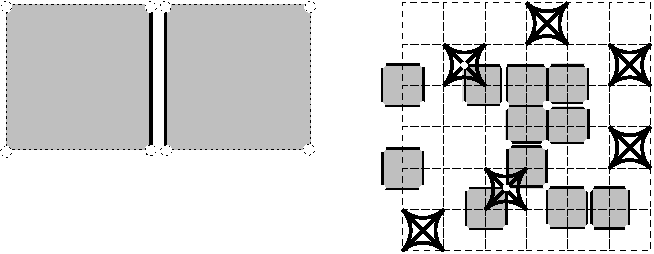
\includegraphics{./Mixed-figs/kanten2}
  \caption{Der zweite Schritt. Links: Zwei besetzte Plaketten, die etwas auseinanderger\"uckt sind, und mit je einer Kopie der Kante als Randst\"uck versehen werden.  Diese Kante hat $\lambda=2$. Alle anderen Randst\"ucke sind noch nicht vorhanden. Rechts ist die Figur aus Abb. \ref{fig:mixed} gezeigt, die um alle Kanten entsprechend der im Text beschrieben Prozedur erweitert wurde. Die Ecken der besetzten Plaketten fehlen noch.}
  \label{fig:kanten}
\end{figure}
Wenn beide angrenzenden dualen Plaketten besetzt sind, m\"ussen diese Plaketten infinitesimal auseinanderger\"uckt und je eine Kopie der dualen Kante von $k$ an beide Plaketten angef\"ugt werden (siehe Abb. \ref{fig:kanten}). Die duale Kante $\bar{k}$ ist dann zweimal in $F$ enthalten. Wir definieren $\lambda(k)$ als die Anzahl der in $F$ vorhandenen Kopien von $\bar{k}$. Seien $v_1(k)$ und $v_2(k)$ die Vertices des urspr\"unglichen Gitters, zwischen denen $k$ liegt. Dann ist 
\begin{equation}
\fbox{$\displaystyle
  \lambda(k):=\begin{cases} \lambda(v_1(k))+ \lambda(v_2(k)) \qquad & \text{falls}\;\; \sigma(k)=0, \\
 1-\left[1-\lambda(v_1(k))\right]\left[1-\lambda(v_2(k))\right] \qquad & \text{falls} \;\; \sigma(k)=1.\end{cases}
$}
\end{equation}
Wenn diese Prozedur an allen Kanten durchgef\"uhrt worden ist, besteht $F$ aus offenen Plaketten und Kanten ohne Randpunkte. Die Ecken der besetzten Plaketten fehlen noch. Die Figur $F$ der Konfiguration aus Abbildung \ref{fig:mixed} ist rechts in Abbildung \ref{fig:kanten} in diesem Zustand gezeigt.

\paragraph{Ecken:} Wenn eine Plakette $f$ des Gitters dekoriert ist, d.h. $\sigma(f)=1$ ist, sind alle Vertices auf dem Rand der Plakette miteinander verbunden. Die dualen Plaketten der Vertices auf dem Rand von $f$ \"uberlappen alle am dualen Vertex $\bar{f}$ von $f$. Wird $\bar{f}$ zu $F$ hinzugef\"ugt, werden daher die geforderten Zusammenhangsverh\"altnisse erzeugt. Sei nun $f$ eine Plakette mit $\sigma(f)=0$. Um die gew\"unschten Zusammenhangsverh\"altnisse zu erzeugen, entfernen wir aus $F$ eine kleine, um die duale Ecke $\bar{f}$ der Plakette $f$ zentrierte, offene Kreisscheibe $B_r(f)$ mit Radius $r$ (siehe links in Abb. \ref{fig:ecken}). Die neue Figur $F_r'(f)$ ist dann
\begin{equation}
  F_r'(f)=F\backslash B_r(f).
\end{equation}
Sei nun $S_r(f)$ ein Kreisring mit Mittelpunkt bei $\bar{f}$ und Radius $r$. Die neu entstandenen Randst\"ucke sind der Durchschnitt von $S_r(f)$ mit $F$ (siehe Abb. \ref{fig:ecken}). Den Durchschnitt bezeichnen wir mit $\Lambda_r(f):=S_r(f)\cap F$. 
\begin{figure}[tbp]
  \centering
  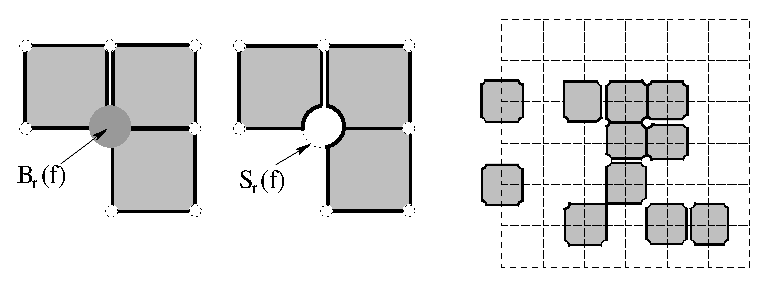
\includegraphics{./Mixed-figs/ecken}
  \caption{Der dritte Schritt: Damit die dualen Plaketten von Vertices auf dem Rand einer undekorierten Plakette $f$ des urspr\"unglichen Gitters nicht zusammenh\"angen, die Figur aber dennoch abgeschlossen ist, wird eine offene Kreisscheibe $B_r(f)$, zentriert an der dualen Ecke $\bar{f}$, entfernt. Die neu entstandenen Randst\"ucke sind der Durchschnitt $\Lambda_r(f)=S_r(f)\cap F$ des Kreises $S_r(f)$ mit $F$. $\Lambda_r(f)$ h\"angt nicht nur von den $\bar{f}$ umgebenden Plaketten ab, sondern auch davon, ob diese verbunden sind oder nicht. Die Euler-Charakteristik $\chi(\Lambda_r)$ ist im dargestellten Fall zwei. Rechts ist die Figur aus Abb. \ref{fig:mixed} dargestellt, nachdem sie an allen Kanten und Ecken modifiziert worden ist. }
  \label{fig:ecken}
\end{figure}
\\Im Limes $r \rightarrow 0$ werden die Beitr\"age der dualen Plaketten und Kanten zu Fl\"ache, Umfang und Euler-Charakteristik nicht ver\"andert. Die Randst\"ucke $\Lambda_r(f)$ tragen f\"ur $r\rightarrow 0$ nur zur skalenunabh\"angigen Euler-Charakteristik bei. Das neue, durch die Modifikation ver\"anderte, $F$ ist
\begin{equation}
  F=\lim_{r\rightarrow 0}F_r'(f),
\end{equation}
und der Beitrag einer Ecke zur Euler-Charakteristik von $F$ ist $\chi(\Lambda_r(f))$.
Seien nun $v_i(f)$ und $k_i(f)$ die Kanten und Plaketten, die die Ecke umgeben. F\"ur jede Ecke $f$ definieren wir  
\begin{equation}
  \lambda(f):= \begin{cases} \chi(\Lambda_r(f)) \qquad & \text{falls} \;\; \sigma(f)=0, \\ 1-\prod_{i=1}^n\left[1-\lambda(v_i(f))\right] \qquad & \text{falls} \;\; \sigma(f)=1.
\end{cases}
\end{equation}
$\Lambda_r(f)$ ist eine Vereinigung von Kreissegmenten. Jeder Schnitt des Kreises mit einer besetzten Plakette ist ein offenes Kreissegment. Der Schnitt des Kreises mit den $\lambda(k_i(f))$-fach vorhanden Kanten $k_i(f)$ sind Punkte, die den Abschluss der offenen Kreissegmente bilden. Daher ist  
 \begin{equation}
\fbox{$\displaystyle
  \lambda(f)= \begin{cases} \sum_{i=1}^n \lambda(k_i(f))-\sum_{i=1}^n\lambda(v_i(f)) \qquad & \text{falls} \;\; \sigma(f)=0, \\ 1-\prod_{i=1}^n\left[1-\lambda(v_i(f))\right] \qquad & \text{falls} \;\; \sigma(f)=1.
\end{cases}
$}
\end{equation}
Diese Prozedur muss f\"ur jede Plakette $f$ durchgef\"uhrt werden. Die Figur, die zur Gitterkonfiguration aus Abbildung \ref{fig:mixed} geh\"ort, ist rechts in Abbildung \ref{fig:ecken} dargestellt. \\
 
Sind alle Modifikationen und Erg\"anzungen durchgef\"uhrt, erh\"alt man f\"ur die Euler-Charakteristik der Figur $F$:
\begin{equation}
\fbox{$\displaystyle
  \chi(F)=\sum_{f}\lambda(f)-\sum_{k}\lambda(k)+\sum_{v}\lambda(v).
$}
\end{equation}
Entsprechend k\"onnen auch Umfang und Fl\"ache durch die Summe der Beitr\"age aller Zellen, jeweils multipliziert mit $\lambda$, ausgerechnet werden.
\\Ist $\sigma(f)$ einer Plakette $f$ gleich 0 und sind alle Vertices und Kanten auf dem Rand von $f$ besetzt, entsteht durch die Modifikation ein Loch. Soll dies vermieden werden, muss $\sigma(f)$ in diesem Fall gleich 1 gesetzt werden. 
\\Die Erwartungswerte der $\lambda$'s werden f\"ur unterschiedliche Perkolationskonfigurationen am Ende dieses Kapitels ausgerechnet. Alle bisher berechneten Euler-Charakteristiken lassen sich durch geeignete Wahl der $\sigma$'s erhalten. 

\section{Gemischte Perkolation in drei Dimensionen}
Ein dreidimensionales Gitter l\"asst sich, anders als die planares Gitter, im Allgemeinen nicht in Zellen zerlegen. Daher betrachten wir ohne Bezug auf ein Gitter eine Tessellation des dreidimensionalen Raumes. Eine Tessellation ist eine Anordnung von nicht \"uberlappenden Polyedern, so dass ihre Vereinigung den gesamten $\mathbb{R}^3$ bedeckt \cite{Weygaert:91}. Die Polyeder bestehen aus ihrem dreidimensionalen Inneren und 0- bis $2$-dimensionalen Randzellen. Mit $C_k$ bezeichnen wir die Menge der $k$-dimensionalen, randlosen Zellen. Die Polyeder werden besetzt, und besetzte Polyeder k\"onnen \"uber gemeinsame Randzellen miteinander verbunden sein. 
\\Wir weisen jedem $c_k\in C_k$, $k\in \{ 0,\ldots, 3\}$, eine Variable $\sigma(c_k)\in \{0,1\}$ zu. F\"ur ein Polyeder $c_3$ bedeutet $\sigma(c_3)=1$, dass $c_3$ besetzt ist. F\"ur $c_k$, $k<3$, bedeutet $\sigma(c_k)=1 $, dass alle Polyeder, deren Rand die Zelle $c_k$ enth\"alt, \"uber $c_k$ verbunden sind. Wenn $\sigma(c_k)=0$ ist sollen diese Polyeder nicht \"uber $c_k$ verbunden sein. Die $\sigma$-Variablen erf\"ullen also die gleiche Funktion wie im zweidimensionalen Fall aus Kapitel \ref{sec:2dmixed}, werden aber anstatt mit Bestandteilen des Gitters, mit Zellen der Tesselation indiziert.
\\Wir konstruieren nun zu einem gegebenen Satz von $\sigma$'s ein geometrisches Objekt, das die geforderten Zusammenhangsverh\"altnisse hat. Zu jeder Zelle $c_k$ wird eine weitere Variable $\lambda(c_k)$ eingef\"uhrt, die die Beitr\"age der Zelle zur Figur beschreibt. Als Resultat erhalten wir die Minkowski-Funktionale $W_\nu(F)$ der so gewonnen Figur $F$. Die Minkowski-Funktionale sind ein vollst\"andiger Satz stetiger, additiver, geometrischer Gr\"o"sen \mbox{(siehe \cite{Mecke:94}).} In drei Dimensionen entsprechen ihnen das Volumen, die Oberfl\"ache, die integrale mittlere Kr\"ummung und die Euler-Charakteristik. Wie sich herausstellen wird, sind die $W_\nu(F)$ die Summe der $W_\nu(c_k)$ der einzelnen Zellen $c_k$, jeweils multipliziert mit einer ganzen Zahl $\lambda(c_k)$. Der Multiplikator $\lambda(c_k)$ l\"asst sich f\"ur $k<3$ immer aus den $\lambda$'s der $c_k$ umgebenden, h\"oherdimensionalen Zellen berechnen. 
\paragraph{Polyeder:}Alle besetzten Polyeder geh\"oren zur Figur $F$. F\"ur alle $c_3\in C_3$ ist $\lambda(c_3)=\sigma(c_3)$, und $F$ besteht anfangs nur aus diesen offenen Polyedern. F\"ur diese offenen Zellen wird, bei den Fl\"achen beginnend, ein Rand konstruiert, so dass die resultierende Figur $F$ die durch die $\sigma$'s vorgegebenen Zusammenhangsverh\"altnisse hat. 
\paragraph{Fl\"achen:}
Wenn f\"ur eine Fl\"ache $c_2$ $\sigma(c_2)=1$ ist, und mindestens einer der beiden Polyeder $c_3^1(c_2)$ und $c_3^2(c_2)$, die $c_2$ als gemeinsame Randfl\"ache haben, besetzt ist, wird $c_2$ zu $F$ hinzugef\"ugt. Im Fall $\sigma(c_2)=0$ wird an die Polyeder, sofern sie besetzt sind, je eine Kopie der Fl\"ache angef\"ugt. Wenn beide Polyeder besetzt sind, muss der Spalt zwischen ihnen infinitesimal ``verbreitert'' werden. Analog zu den Kanten im zweidimensionalen Fall gilt f\"ur die $\lambda(c_2)$ einer Fl\"ache $c_2$
\begin{equation}
\fbox{$\displaystyle  \lambda(c_2):=\begin{cases} \lambda(c_3^1(c_2))+ \lambda(c_3^2(c_2)) \qquad & \text{falls}\;\; \sigma(c_2)=0, \\
 1-\left[1-\lambda(c_3^1(c_2))\right]\left[1-\lambda(c_3^2(c_2))\right] \qquad & \text{falls} \;\; \sigma(c_2)=1.\end{cases}$}
\end{equation}
Diese Prozedur wird an allen Fl\"achen durchgef\"uhrt.
\paragraph{Kanten:} Eine Kante $c_1$ wird zu $F$ hinzugef\"ugt, wenn $\sigma(c_1)=1$ ist und mindestens einer der Polyeder $c_3^i(c_1)$, $i=1,\ldots,n$, in deren Rand $c_1$ ist, besetzt ist. Gegebenenfalls muss die Umgebung der Kante derart deformiert werden, dass das Hinzuf\"ugen der Kante alle umliegenden Polyeder und Fl\"achen verbindet (siehe Abb. \ref{fig:kante3d}). Im Fall $\sigma(c_1)=0$ muss $F$ entlang $c_1$ modifiziert werden, denn $c_1$ darf die Polyeder $c_3^i(c_1)$ nicht verbinden. $F$ muss aber entlang $c_1$ abgeschlossen sein. Dazu betrachten wir die offene Kreisscheibe $B_r(c_1)$ mit Radius $r$, die senkrecht auf $c_1$ steht. Der Mittelpunkt von $B_r(c_1)$ sei am Ursprung. Die Minkowskisumme der randlosen Zelle $c_1$ mit $B_r(c_1)$ wird aus $F$ entfernt. Die Minkowskisumme $B_r(c_1)\uplus c_1$ ist die Menge, die entsteht, wenn der Mittelpunkt von $B_r(c_1)$ an jeden Punkt von $c_1$ angeheftet wird (siehe Abb. \ref{fig:minkowski} und \cite{Mecke:94}). 
\begin{figure}[bt]
  \centering
  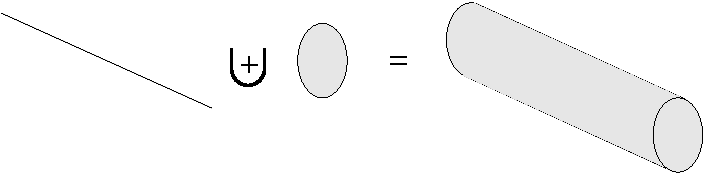
\includegraphics{./Mixed-figs/minkowski}
  \caption{Minkowskisumme einer Kante mit einer Kreisscheibe.}
  \label{fig:minkowski}
\end{figure}
\begin{figure}[bt]
  \centering
  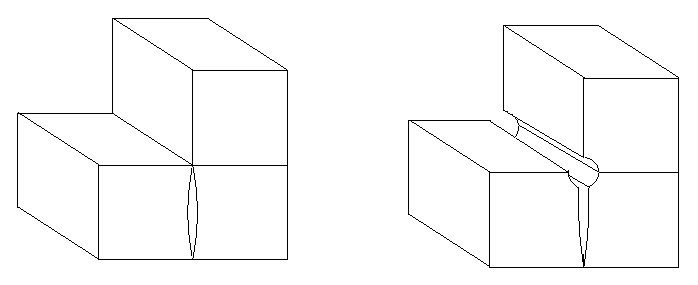
\includegraphics{./Mixed-figs/kante3d}
  \caption{Links sind drei W\"urfel dargestellt, deren gemeinsame Kante $c_1$ $\sigma(c_1)=1$ hat. Die beiden unteren W\"urfel sind nicht \"uber eine Fl\"ache verbunden, aber an der Kante $c_1$. Rechts sind die gleichen W\"urfel mit $\sigma(c_1)=0$ gezeigt. Der Durchschnitt eines hinreichend kleinen Kreises, angeheftet an die Kante, mit der Umgebung, ist in jedem Punkt der Kante gleich. Nur an den Randbereichen der Kante gilt das i. A. nicht. Diese Bereiche verschwinden aber mit dem Radius des Kreises. }
  \label{fig:kante3d}
\end{figure}
Die Menge $F'_r(c_k):=F\backslash(B_r(c_k)\uplus c_k)$ ist entlang $c_1$ abgeschlossen, und die umliegenden Polyeder h\"angen nicht \"uber $c_1$ zusammen (siehe Abb. \ref{fig:kante3d}).  
\\Um $W_\nu(F'_r(c_k))$ zu berechnen, betrachten wir den Kreisring $S_r(c_1)$. Die Vereinigung von $S_r(c_1)$ mit der offenen Kreisscheibe $B_r(c_1)$ ist die abgeschlossene Kreisscheibe $\bar{B}_r(c_1)$.  Mit $S_r(c_1)$ und $\bar{B}_r(c_1)$ l\"asst sich $F'_r(c_1)$ als disjunkte Vereinigung der modifizierten Figur $F$ mit den neuen Randst\"ucken schreiben: 
\begin{equation}
  F'_r(c_1)=\left( F\backslash (\bar{B}_r(c_1) \uplus c_1)\right) \cup \left( F\cap (S_r(c_1)\uplus c_1)\right).
\end{equation}
Wegen der Additivit\"at der Minkowski-Funktionale gilt  
\begin{equation}
\label{eq:modifikation}
  W_\nu(F'_r(c_1))=W_\nu\left(F\backslash(\bar{B}_r(c_1)\uplus c_1)\right)+W_\nu\left(F\cap (S_r(c_1) \uplus c_1)\right).
\end{equation}
Wegen der Stetigkeit der Minkowski-Funktionale gilt im Limes $r \rightarrow 0$ f\"ur den ersten Term auf der rechten Seite von Gleichung (\ref{eq:modifikation}) $W_\nu(F\backslash(\bar{B}_r(c_1)\uplus c_1))\rightarrow W_\nu(F\backslash c_1)=W_\nu(F)$. Die Beitr\"age der Polyeder und Fl\"achen werden durch die Modifikation im Limes $r\rightarrow 0$ also nicht ver\"andert, und alle zus\"atzlichen Beitr\"age kommen von den neuentstandenen Randst\"ucken entlang $c_1$. 
\\Im Limes $r\rightarrow 0$ ist $F\cap (S_r(c_1)\uplus x)$ mit $x\in c_1$ f\"ur alle $x$ gleich (abgesehen von einer Translation, siehe Abb. \ref{fig:kante3d}), und es gibt ein $\Lambda_r(c_1)$, so dass $F\cap (S_r(c_1)\uplus c_1)=\Lambda_r(c_1)\uplus c_1$ gilt. $\Lambda_r(c_1)$ ist die an den Ursprung verschobene Menge $F\cap (S_r(c_1)\uplus x)$.
Da $\Lambda_r(c_1)$ und $c_1$ in komplement\"aren, orthogonalen Unterr\"aumen liegen, ist die Formel $51$, Kapitel $6$ aus \cite{Hadwinger:57} anwendbar, und man erh\"alt f\"ur den zweiten Term in Gleichung (\ref{eq:modifikation})
\begin{equation}
  \label{eq:hadwinger}
  W_{\nu}(c_1\uplus\Lambda_r(c_1))=\frac{\omega_{\nu}}{{d \choose \nu}}\sum_{\mu=0}^{\nu}{k\choose \mu}{d-k \choose \nu-\mu}\frac{W'_{\mu}(c_1)W'_{\nu-\mu}(\Lambda_r(c_1))}{\omega_{\mu}\omega_{\nu-\mu}}.
\end{equation}
Im Limes $r \rightarrow 0$ verschwinden alle skalenabh\"angigen  $W'_{\nu-\mu}(\Lambda_r(c_1))$ und obige Formel vereinfacht sich zu 
\begin{equation}
 \lim_{r \rightarrow 0} W_{\nu}(c_1\uplus\Lambda_r(c_1))=W_{\nu}(c_1)\chi(\Lambda(c_1)).
\end{equation}
Damit wird aus Gleichung (\ref{eq:modifikation}) im Limes $r \rightarrow 0$
\begin{equation}
 \lim_{r\rightarrow 0} W_\nu(F'_r(c_1))=W_\nu\left(F\right)+W_\nu(c_1)\chi(\Lambda(c_1)).
\end{equation}
Die Euler-Charakteristik $\chi(\Lambda_r(c_1))$ ist unabh\"angig vom Radius $r$, der daher weggelassen wird. Die Beitr\"age der Modifikation zu den Minkowski-Funktionalen sind also die Minkowski-Funktionale der Zelle $c_1$, multipliziert mit der ganzen Zahl $\chi(\Lambda(c_1))$. Die Multiplizit\"at der Kante $c_1$ wird durch 
\begin{equation}
\fbox{$ \displaystyle 
  \lambda(c_1):= \begin{cases} \chi(\Lambda(c_1)) \qquad & \text{falls} \;\; \sigma(c_1)=0, \\ 1-\prod_{i=1}^n\left[1-\lambda(c_3^i(c_1))\right] \qquad & \text{falls} \;\; \sigma(c_1)=1,
\end{cases}
$}
\end{equation}
definiert. $\Lambda(c_1)$ ist der Durchschnitt eines Kreisrings mit den besetzten Polyedern $c_3^i(c_1)$ und den zwischen ihnen liegenden $\lambda(c_2^1(c_1))$-fach vorhandenen Fl\"achen $c_2^i(c_1)$. $\Lambda(c_1)$ liegt in einer Ebene senkrecht auf $c_1$, und die entstehenden Schnittmuster sind Kreissegmente, analog zu dem Schnitt eines Kreises mit den dualen Plaketten und Kanten, die eine duale Ecke des zweidimensionalen Gitters umgeben (siehe Abb. \ref{fig:ecken}). Jeder Schnitt mit einem besetzten Polyeder ist ein offenes Kreissegment, und die Schnitte mit den Fl\"achen liefern je $\lambda(c_2^i(c_1))$ Punkte. Die Euler-Charakteristik von $\Lambda(c_1)$ ist daher
 \begin{equation}
 \chi(\Lambda(c_1))= \sum_{i=1}^n \lambda(c_2^i(c_1))-\sum_{i=1}^n\lambda(c_3^i(c_1)).
\end{equation}   
Die Figur $F$ wird jetzt durch $\lim_{r\rightarrow 0}F'_r(c_k)$ ersetzt, und die Prozedur nacheinander an allen Kanten durchgef\"uhrt. 
\paragraph{Ecken:} Eine Ecke $c_0$ der Tesselation wird von Polyedern $c_3^1(c_0),\ldots,c_3^n(c_0)$, Fl\"achen $c_2^1(c_0),$ \ldots,$c_2^m(c_0)$ und Kanten $c_1^1(c_0),\ldots,c_1^l(c_0)$ umgeben. Ist $\sigma(c_0)=1$ und mindestens einer der umgebenden Polyeder besetzt, wird $c_0$ zu $F$ hinzugef\"ugt und verbindet die offenen Enden an der Ecke. Dazu ist gegebenfalls eine Deformation der Umgebung der Ecke n\"otig. Falls $\sigma(c_0)=0$ ist, wird eine offene Kugel $B_r(c_0)$ mit Radius $r$, zentriert bei $c_0$, aus $F$ entfernt. Wie im Fall einer Kante werden die Beitr\"age der h\"oherdimensionalen umgebenden Zellen zu den Minkowskifunktionalen im Limes $r\rightarrow 0$ nicht ver\"andert. Die neuen Randst\"ucke sind der Schnitt einer Sph\"are $S_r(c_0)$ mit $F$. Die Randst\"ucke $\Lambda_r(c_0)=S_r(c_0)\cap F$ tragen im Limes $r\rightarrow 0$ nur zur Euler-Charakteristik bei, und wir definieren $\lambda(c_0)$ durch $\chi(\Lambda_r(c_0))$. $\Lambda_r(c_0)$ besteht aus dem Schnitt von $S_r(c_0)$ mit den umgebenden besetzten Polyedern, den dazwischenliegenden $\lambda(c_2^i(c_0))$-fach vorhandenen Fl\"achen und den, gegebenenfalls modifizierten, Kanten. Jeder Schnitt mit einem besetzten Polyeder ist ein offenes Gebiet auf der Sph\"are und liefert den Beitrag $+1$. Der Schnitt mit einer $\lambda(c_2^i(c_0))$-fach vorhandenen Fl\"ache sind $\lambda(c_2^i(c_0))$ offene Geradenst\"ucke, die $-\lambda(c_2^i(c_0))$ zur Euler-Charakteristik beitragen. Der Schnitt der Sph\"are mit einer Kante ist ein Punkt und tr\"agt $+1$ bei. Die Umgebung von Kanten mit $\sigma(c_1^i(c_0))=0$ wurde aber modifiziert, und der Schnitt mit den durch die Modifikation entstandenen Randst\"ucken ist gerade $\lim_{r\rightarrow 0}\Lambda_r(c_1^i(c_0))$. Die Kanten tragen also $\lambda(c_1^i(c_0))$ zu Euler-Charakteristik bei. Damit ergibt sich: 
\begin{equation}
\label{eq:lambdaecken}
\fbox{$ \displaystyle 
  \lambda(c_0):= \begin{cases} \sum_{i=1}^n \lambda(c_3^i(c_0))-\sum_{i=1}^m\lambda(c_2^i(c_0))+\sum_{i=1}^l\lambda(c_1^i(c_0))\qquad & \text{falls} \;\; \sigma(c_0)=0, \\ 1-\prod_{i=1}^n\left[1-\lambda(c_3^i(c_0))\right] \qquad & \text{falls} \;\; \sigma(c_0)=1.
\end{cases}
$}
\end{equation}
Nachdem $F$ an allen Ecken auf diese Weise modifiziert wurde, ist $F$ abgeschlossen und hat die geforderten Zusammenhangsverh\"altnisse.
\\Die Minkowski-Funktionale von $F$ sind dann die Summe der Beitr\"age der einzelnen Zellen $c$, jeweils multipliziert mit der ganzen Zahl $\lambda(c)$:
\begin{equation}
\fbox{$\displaystyle
  W_{\nu}(F,\{\mathbf{\sigma}\})=\sum_{c}\lambda(c)W_{\nu}(c)
$}
\end{equation}

Wenn $\sigma(c_k)$ einer $k$-Zelle $c_k$ gleich null ist und alle umliegenden h\"oherdimensionalen Zellen $\sigma=1$ haben, wird durch die Modifikation ein $k$-dimensionaler Tunnel erzeugt. Wenn solche Tunnel vermieden werden sollen, muss $\sigma(c_k)$ in diesem Fall auf den Wert 1 gesetzt werden. 
\\

Die formale Behandlung der Modifikation an den Kanten l\"asst sich ohne weiteres auf die Fl\"achen und Ecken \"ubertragen. In entsprechender Weise kann der Formalismus auch auf $d$-dimensionale Tesselationen verallgemeinert werden. Da dies in dieser Arbeit nicht ben\"otigt wird, beschr\"anken wir uns auf zwei und drei Dimensionen.  

\section{Anwendung auf Perkolationskonfigurationen}

\subsection{bond-site Perkolation}
\label{sec:bond-site}
Bei bond-site-Perkolation werden Vertices eines Gitters mit Wahrscheinlichkeit $p_s$ und Kanten des Gitters mit Wahrscheinlichkeit $p_b$ besetzt. Wir wenden nun den oben erarbeiteten Formalismus auf bond-site-Perkolation in drei Dimensionen an und betrachten dazu ein Gitter, zu dem Zellen existieren, deren Fl\"achen den Gitterkanten entsprechen. Diese Zellen bilden die Tesselation aus dem vorhergehenden Abschnitt.
\\Jede dreidimensionale Zelle $c_3$ wird mit Wahrscheinlichkeit $p_s$ besetzt, d.h. mit Wahrscheinlichkeit $p_s$ ist $\sigma(c_3)=1$. Die Fl\"achen entsprechen den Gitterkanten und $\sigma$ jeder Fl\"ache wird mit Wahrscheinlichkeit $p_b$ auf den Wert 1 gesetzt. Die $\sigma$-Variablen der Kanten und Ecken haben den Wert 0, sofern nicht alle umliegenden $3$-Zellen und Fl\"achen $\sigma=1$ haben. Dadurch wird gew\"ahrleistet, dass entlang der Kanten und Ecken keine Tunnel bzw. Einschl\"usse entstehen, wenn alle umliegenden $3$-Zellen und Fl\"achen besetzt sind. Um die Erwartungswerte der $W_\nu$ zu berechnen, m\"ussen wir die Erwartungswerte $\left<\lambda(c)\right>_{p_s,p_b}$ aller Zellen kennen.
\\Der Erwartungswert $\left<\lambda_3\right>_{p_s,p_b}$ einer beliebigen $3$-Zelle ist $p_s$. Der Erwartungswert $\left<\lambda(c_2)\right>_{p_s,p_b}$ einer Fl\"ache $c_2$ setzt sich aus einem Beitrag mit $\sigma(c_2)=1$ und einem mit $\sigma(c_2)=0$ zusammen. Im ersten Fall ist $\lambda(c_2)=1$, wenn immer eine der angrenzenden $3$-Zellen besetzt ist; im zweiten Fall ist $\lambda(c_2)$ die Zahl der besetzten angrenzenden $3$-Zellen. F\"ur jede Fl\"ache $c_2$ gilt daher 
\begin{equation}
  \left<\lambda(c_2)\right>_{p_s,p_b}=\left<\lambda_2\right>_{p_s,p_b}=(1-(1-p_s)^2)p_b+2p_s(1-p_b)=2p_s-p_bp_s^2.
\end{equation}
Eine Kante $c_1$ umgeben die $3$-Zellen $c_3^1(c_1),\ldots,c_3^n(c_1)$ und die Fl\"achen $c_2^1(c_1),\ldots,c_2^n(c_1)$. Auch bei Kanten m\"ussen die F\"alle  $\sigma(c_1)=1$ und  $\sigma(c_1)=0$ unterschieden werden. Der erste Fall tritt mit der Wahrscheinlichkeit $p_s^np_b^n$ ein. Im zweiten Fall m\"ussen wir immer voraussetzen, dass nicht f\"ur alle $i\in \{1,\ldots,n\}$  $\sigma(c_3^i(c_1))=\sigma(c_2^i(c_1))=1$ gilt. Daher sind die Beitr\"age der einzelnen Fl\"achen und $3$-Zellen zu $\lambda(c_1)$ nicht mehr unabh\"angig und m\"ussen einzeln abgez\"ahlt werden. Zum Abz\"ahlen aller m\"oglichen Zust\"ande der umgebenden 3-Zellen und Fl\"achen und zur Berechnung der $\lambda(c_1)$ habe ich ein Computerprogramm (siehe dazu Anhang \ref{sec:noofcomp}) geschrieben.  
\\Eine Ecke $c_0$ sei von den $3$-Zellen $c_3^1(c_0),\ldots,c_3^m(c_0)$, den Fl\"achen $c_2^1(c_0),\ldots,c_2^n(c_0)$ und den Kanten $c_1^1(c_0),\ldots,c_1^l(c_0)$ umgeben. Wenn $\sigma(c_3^i(c_0))=1$ f\"ur alle $i\in \{1,\ldots,m\}$ und $\sigma(c_2^i(c_0))=1$ f\"ur alle $i\in \{1,\ldots,n\}$ gilt, ist $\sigma(c_0)=1$. Anderfalls, muss $\chi(\Lambda(c_0))$ berechnet werden. Hierzu werden wieder alle m\"oglichen Zust\"ande der umgebenden Zellen und Fl\"achen abgez\"ahlt und jeweils $\lambda(c_0)$ berechnet.
\\Da die Berechnung der $\left<\lambda_3\right>_{p_s,p_b}$, $\left<\lambda_2\right>_{p_s,p_b}$ und $\left<\lambda_1\right>_{p_s,p_b}$ in drei Dimensionen der Berechnung der $\left<\lambda_2\right>_{p_s,p_b}$, $\left<\lambda_1\right>_{p_s,p_b}$ bzw. $\left<\lambda_0\right>_{p_s,p_b}$ in zwei Dimensionen entspricht, kann bond-site-Perkolation auf zweidimensionalen Gittern v\"ollig analog behandelt werden. 


\subsubsection{Euler-Charakteristik der bond-site-Perkolation auf dem Quadratgitter}
\label{sec:bondsitesq}
Um die Euler-Charakteristik der bond-site-Perkolation auf dem Quadratgitter zu erhalten, muss nur noch $\left<\lambda(c_0)\right>_{p_s,p_b}$ jeder dualen Ecke $c_0$ bestimmt werden. Alle Ecken des Quadratgitters werden von vier Quadraten umgeben. Daher ist $\left<\lambda(c_0)\right>_{p_s,p_b}$ einer Ecke $c_0$ f\"ur alle Ecken gleich $\left<\lambda_0\right>_{p_s,p_b}$. 
Alle m\"oglichen Konfigurationen der vier Quadrate und Kanten werden abgez\"ahlt, und die $\lambda_0$ mit ihrer Wahrscheinlichkeit gewichtet und aufsummiert. Man erh\"alt 
\begin{equation}
    \left<\lambda_0\right>_{p_s,p_b} = 4p_s+p_b^4p_s^4-4p_bp_s^2.
\end{equation}
Die mittlere Euler-Charakteristik der bond-site-Perkolation auf dem Quadratgitter ist damit:
\begin{equation}
  \label{eq:bondsitesq}
  \fbox{$ \chi(p_s,p_b)=p_s-2p_bp_s^2+p_b^4p_s^4.$}
\end{equation}
\subsubsection{Euler-Charakteristik der bond-site-Perkolation auf dem einfach kubischen Gitter}
\label{sec:bondsitesc}
Die Zellen des einfach kubischen Gitters (sc-Gitter) sind W\"urfel. Da jede Kante von vier W\"urfeln umgeben ist, gilt f\"ur das sc-Gitter, analog zum zweidimensionalen Quadratgitter,
\begin{eqnarray} 
  \left<\lambda_3\right>_{p_s,p_b} &=& p_s,\\
  \left<\lambda_2\right>_{p_s,p_b} &=& 2p_s-p_bp_s^2,\\
  \left<\lambda_1\right>_{p_s,p_b} &=& 4p_s+p_b^4p_s^4-4p_bp_s^2.
\end{eqnarray}
Eine W\"urfelecke ist von acht W\"urfeln, zw\"olf Fl\"achen und sechs Kanten umgeben. Zu jeder m\"oglichen Konfiguration muss $\lambda_0$ aus den $\lambda$'s aller W\"urfel, Fl\"achen und Kanten bestimmt werden. 
Die Summation aller Beitr\"age liefert 
\begin{equation}
\left<\lambda_0\right>_{p_s,p_b}=8p_s-12p_bp_s^2+6p_b^4p_s^4-p_b^{12}p_s^8.
\end{equation}
Pro W\"urfel gibt es je drei Fl\"achen und Kanten, sowie eine Ecke, und f\"ur die Euler-Charakter\-istik (siehe Abb.  \ref{fig:chi-bond-site}) erh\"alt man  
\begin{equation}
  \label{eq:bondsitesc}
\fbox{$
\begin{split}
\chi(p_s,p_b)&=  \left<\lambda_0\right>_{p_s,p_b}-3\left<\lambda_1\right>_{p_s,p_b}+3\left<\lambda_2\right>_{p_s,p_b}-\left<\lambda_3\right>_{p_s,p_b}\\
&= p_s-3p_s^2p_b+3p_s^4p_b^4-p_s^8p_b^{12}.
\end{split}$}
\end{equation}\\

Die mittleren Euler-Charakteristiken des Quadrat- (Gl. \ref{eq:bondsitesq}) und des sc-Gitters (Gl. \ref{eq:bondsitesc}) sind f\"ur $p_s=0$ konstant null, da ein Cluster mindestens einen besetzten Vertex enthalten muss, und daher f\"ur $p_s=0$ keine Cluster existieren (siehe Abb. \ref{fig:chi-bond-site}). 
\begin{figure}[bt]
  \centering
  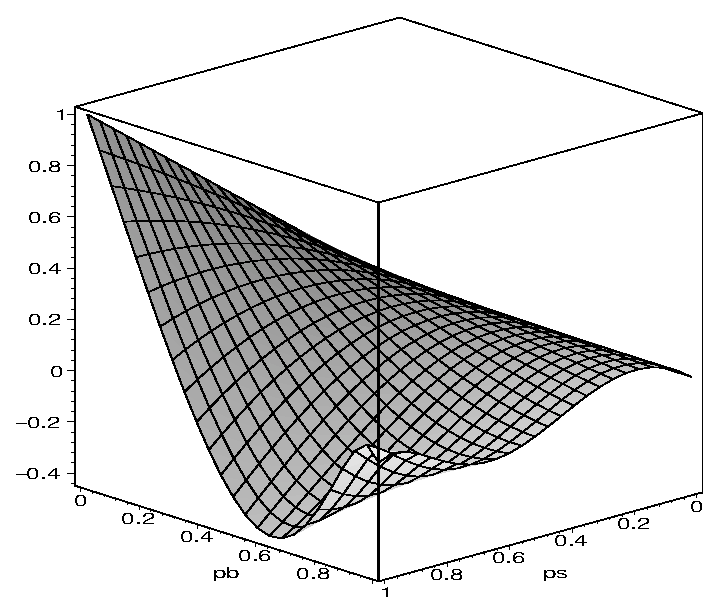
\includegraphics{./Mixed-figs/chibondsiteplot}
  \caption{Euler-Charakteristik $\chi(p_s,p_b)$ der bond-site-Perkolation auf dem sc-Gitter.}
  \label{fig:chi-bond-site}
\end{figure}
F\"ur $p_b=0$ besteht die Anordnung aus isolierten abgeschlossenen Zellen und $\chi(p_s,0)=p_s$. Der Fall $p_b=1$ wird die Euler-Charakteristik der site-Perkolation auf dem Quadrat- bzw. sc-Gitter reproduziert. F\"ur $p_s=1$ ist $\chi(p_s=1,p_b)$ die Euler-Charakteristik des reinen bond-Perkolationsprozesses des Quadrat- bzw. sc-Gitters. 

\subsection{Euler-Charakteristik des bcc-Gitters}
\label{sec:mixedbcc}
Neben der Berechnung der Euler-Charakteristik von bond-site-Perkolationsprozessen eignet sich der vorgestellte Formalismus auch, um bei reinen site-Perkolationsproblemen bestimmte Nachbarschaftsverh\"altnisse zu erzwingen, wenn keine geeigneten Zellen mit den Nachbarschaftsverh\"altnissen des Gitters gefunden werden k\"onnen. Am Beispiel der Wigner-Seitz-Zelle (WSZ) des bcc-Gitter soll eine solche Anwendung hier vorgef\"uhrt werden. Die WSZ des bcc-Gitters hat 14 Fl\"achen, ein Gittervertex aber nur acht n\"achste Nachbarn. Um eine mittlere Euler-Charakteristik zu erhalten, die der 8-Nachbarschaft entspricht, k\"onnen entweder komplizierte nicht konvexe Zellen (siehe Abb. \ref{fig:bcc_nonconvex_app}) gew\"ahlt werden, oder auf den Fl\"achen der WSZ die $\sigma$'s entsprechend der 8-Nachbarschaft vorgegeben werden (siehe Abb. \ref{fig:bccconvexapp}). Die sechseckigen Fl\"achen entsprechen Gitternachbarschaften und haben $\sigma=1$. Die Quadrate entsprechen keinen Gitternachbarschaften und haben $\sigma=0$, falls die beiden angrenzenden Zellen keinen gemeinsamen besetzten Gitternachbarn haben. Andernfalls ist $\sigma=1$. 
\begin{figure}[htbp]
  \centering
  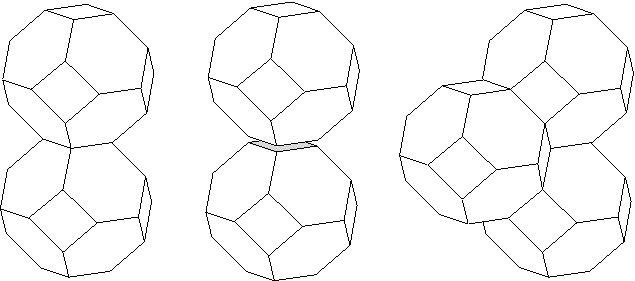
\includegraphics{./Mixed-figs/bcc_nn}
  \caption{WSZ des bcc-Gitter gelten nur als benachbart, wenn sie n\"achste Nachbarn sind (sechseckige Fl\"achen) oder einen gemeinsamen n\"achsten Nachbar haben: Zwei WSZ die sich an einem Quadrat ber\"uhren (links), werden getrennt (Mitte), solange sie keinen gemeinsamen n\"achsten Nachbar haben (rechts).}
  \label{fig:bccconvexapp}
\end{figure}
WSZ werden mit Wahrscheinlichkeit $p=1-q$ besetzt, und $\left<\lambda_3\right>_{p}=p$. F\"ur Sechsecke gilt $\left<\lambda_2^{hex}\right>_{p}=1-q^2=2p-p^2$. F\"ur ein Quadrat ist $\lambda_2^{sq}=1$, wenn genau eine der beiden angrenzenden WSZ besetzt ist. Wenn beide besetzt sind, ist $\lambda_2^{sq}=1$, wenn mindestens einer der vier gemeinsamen Nachbarn besetzt ist, und anderfalls $\lambda_2^{sq}=2$. F\"ur den Erwartungswert erh\"alt man
\begin{equation}
 \left<\lambda_2^{sq}\right>_{p}=2pq+p^2(1-q^4)+2p^2q^4=2pq+p^2(1+q^4).
\end{equation}
Jede Kante $c_1$ ist im Rand eines Quadrates und zweier Sechsecke enthalten. Sobald mindestens eine der umliegenden Zellen besetzt ist, ist die Kante vorhanden. Nur wenn das Quadrat $\lambda=2$ hat, ist $\lambda(c_1)=2$ und man erh\"alt
\begin{equation}
 \left<\lambda_1\right>_{p}=(1-q^3)+p^2q^4. 
\end{equation}
Eine Ecke $c_0$ geh\"ort zu vier Zellen, von denen zwei Paare keine Gitternachbarn sind. Die Ecke ist vorhanden, wenn mindestens eine der vier Zellen besetzt ist. $\lambda(c_0)=2$, wenn zwei WSZ besetzt sind, die keine n\"achsten Nachbarn sind, und gleichzeitig keine der vier gemeinsamen Gitternachbarn besetzt sind. Daher ist
\begin{equation}
 \left<\lambda_0\right>_{p}=(1-q^4)+2p^2q^4. 
\end{equation}
Es gibt pro Zelle acht Sechsecke und sechs Quadrate, die je zu zwei Zellen geh\"oren, 36 Kanten, die zu drei Zellen geh\"oren, und 24 Ecken, die zu vier Zellen geh\"oren. F\"ur die Euler-Charakteristik pro Zelle oder Gittervertex ergibt sich mit dieser Methode
\begin{equation}
  \chi^{bcc}_{8-14}(p)=p-4p^2+12p^4-12p^5+3p^6.
\end{equation}

\subsection{Weitere Anwendungsm\"oglichkeiten}
Der vorgestellte Formalismus l\"asst sich auf jeden beliebigen Satz von $\sigma$-Variablen anwenden, und somit ist es m\"oglich, geometrische Eigenschaften von Figuren zu berechnen, deren Konstituenten auf unterschiedlichste Weise zusammenh\"angen. Insbesondere ist es auch vorstellbar, wechselwirkende Modelle zu betracheten, und topologische Fluktuationen in Mikroemulsionen zu behandeln \cite{Jung:00}. Topologischen Fluktuationen k\"onnen sowohl Euler-Charakteristik, als auch integrale mittlere Kr\"ummung und Oberfl\"ache, ver\"andern, und Beitr\"age zu den thermodynamischen Potentialen der Mikroemulsion liefern \cite{Likos:95}. Dadurch wird sich das Phasendiagramm der Mikroemulsion ver\"andern und unter Umst\"anden zu neuen Phasen f\"uhren.
